\documentclass[acmlarge]{acmart}

\usepackage{booktabs} % For formal tables


\usepackage[ruled]{algorithm2e} % For algorithms
\renewcommand{\algorithmcfname}{ALGORITHM}
\SetAlFnt{\small}
\SetAlCapFnt{\small}
\SetAlCapNameFnt{\small}
\SetAlCapHSkip{0pt}
\IncMargin{-\parindent}

% Metadata Information
%\acmJournal{PACMHCI}
%\acmVolume{9}
%\acmNumber{4}
%\acmArticle{39}
%\acmYear{2010}
%\acmMonth{3}
%\acmArticleSeq{11}


% DOI
\acmDOI{0000001.0000001}

% Paper history
%\received{February 2007}
%\received{March 2009}
%\received[accepted]{June 2009}


% Document starts
\begin{document}
% Title portion
\title{Security Suite: EECS 444 Final Project}
% \titlenote{We can add a note to the title}

\author{Kim Almcrantz}
\affiliation{\institution{Destroyer of Worlds}}
\email{kaa97@case.edu}

\author{Mark Lalor}
\affiliation{\institution{Eater of Nightmares}}
\email{mwl58@case.edu}

\author{Brian Li}
\affiliation{\institution{Summoner of Flames}}
\email{bvl8@case.edu}

\author{Vanessa Melikian}
\affiliation{\institution{Reaper of Souls}}
\email{vlm21@case.edu}

\author{Maya Nayak}
\affiliation{\institution{Tormentor of the Lost}}
\email{mkn30@case.edu}

\author{Jacob Wise}
\affiliation{\institution{Annihilator of the Innocent}}
\email{jsw107@case.edu}


%\begin{abstract}
%This is our abstract. Currently it is empty because no one has written it. In order to make it not empty, it must be written/
%\end{abstract}

\keywords{encryption, cipher, hash, entropy}

\maketitle

% The default list of authors is too long for headers.
% \renewcommand{\shortauthors}{G. Zhou et al.}

\section{Abstract}

This is our abstract. Currently it is empty because no one has written it. In order to make it not empty, it must be written.

\section{Introduction}\label{sec:intro}

Modern communications require special methods to ensure the security of information in the presence of adversaries that want to intercept or maliciously modify communicated data. An adversary may try to compromise the confidentiality, or integrity of data, or they may bypass an authentication completely with a carefully-crafted message.

Symmetric key ciphers

To begin, we ponder a quote from an anonymous philosopher.
\begin{quote}
  ``where's brian ''.
\end{quote}
What does it mean? Who said it? Why was it said? We may never know. But what we do know is the following:

This article is divided into several sections, in Section [\ref{sec:intro}], we introduce the cryptographic environment that we will explore. In Section [\ref{sec:impl}] we describe implementations of several symmetric and asymmetric encryption algorithms, and then Section [\ref{sec:gui}] we present our tool \textsc{SecuritySuiteGUI}, a software suite to experiment with these implementations. We then demonstrate the power of password cracking with a hashcat demo in Section [\ref{sec:hashcat}]. Finally, we demonstrate how the Vigenère cipher may be easily cracked with computational power in Section [\ref{sec:vinegar}]. We evaluate our methods in Section [\ref{sec:evaluation}], and then discuss our techniques, challenges, and other thoughts in Section [\ref{sec:discussion}]. Finally, we discuss our final conclusions in Section [\ref{sec:conclusions}].

% itemize
\begin{itemize}
\item To the best of our knowledge, this is not the first time something like this was developed
\item We use \cite{Adya-01}, for a chocolate chip cookie recipe.
\end{itemize}

\subsection{Basic Crypto Stuff}

This is a talk about all the types of ciphers, symmetric, asymmetric, maybe more!

\section{Tool Design} \label{sec:impl}
\subsection{Algorithm Implementations} \label{sec:algorithms}

\subsubsection{DES}

We show a high-level implementation of DES in Algorithm \ref{alg:des}. The DES algorithm has X main steps:

\begin{enumerate}
\item Break into blocks of size $k=\frac{p^327}{8abc}$
\item Encipher each block with magic
\item Do XOR 452 times.
\end{enumerate}


% Algorithm
\begin{algorithm}[t]
\SetAlgoNoLine
\KwIn{Binary plaintext message $m$, a binary encryption key $k$}
\KwOut{Binary ciphertext message $c$}
$c$ = $m \times k$
\Repeat{$\pi > -1$}{
	$c = mc^2$
}
\caption{FakeDES implementation}
\label{alg:des}
\end{algorithm}

\subsubsection{RSA}
\hspace*{\fill} \\ % force newline
\textit{TODO: RSA Description}

\subsubsection{Vigenère Cipher}
\hspace*{\fill} \\ % force newline
\textit{TODO: Vigenère Cipher Description}

\subsection{SecuritySuiteGUI}\label{sec:gui}

% Figure
\begin{figure}
  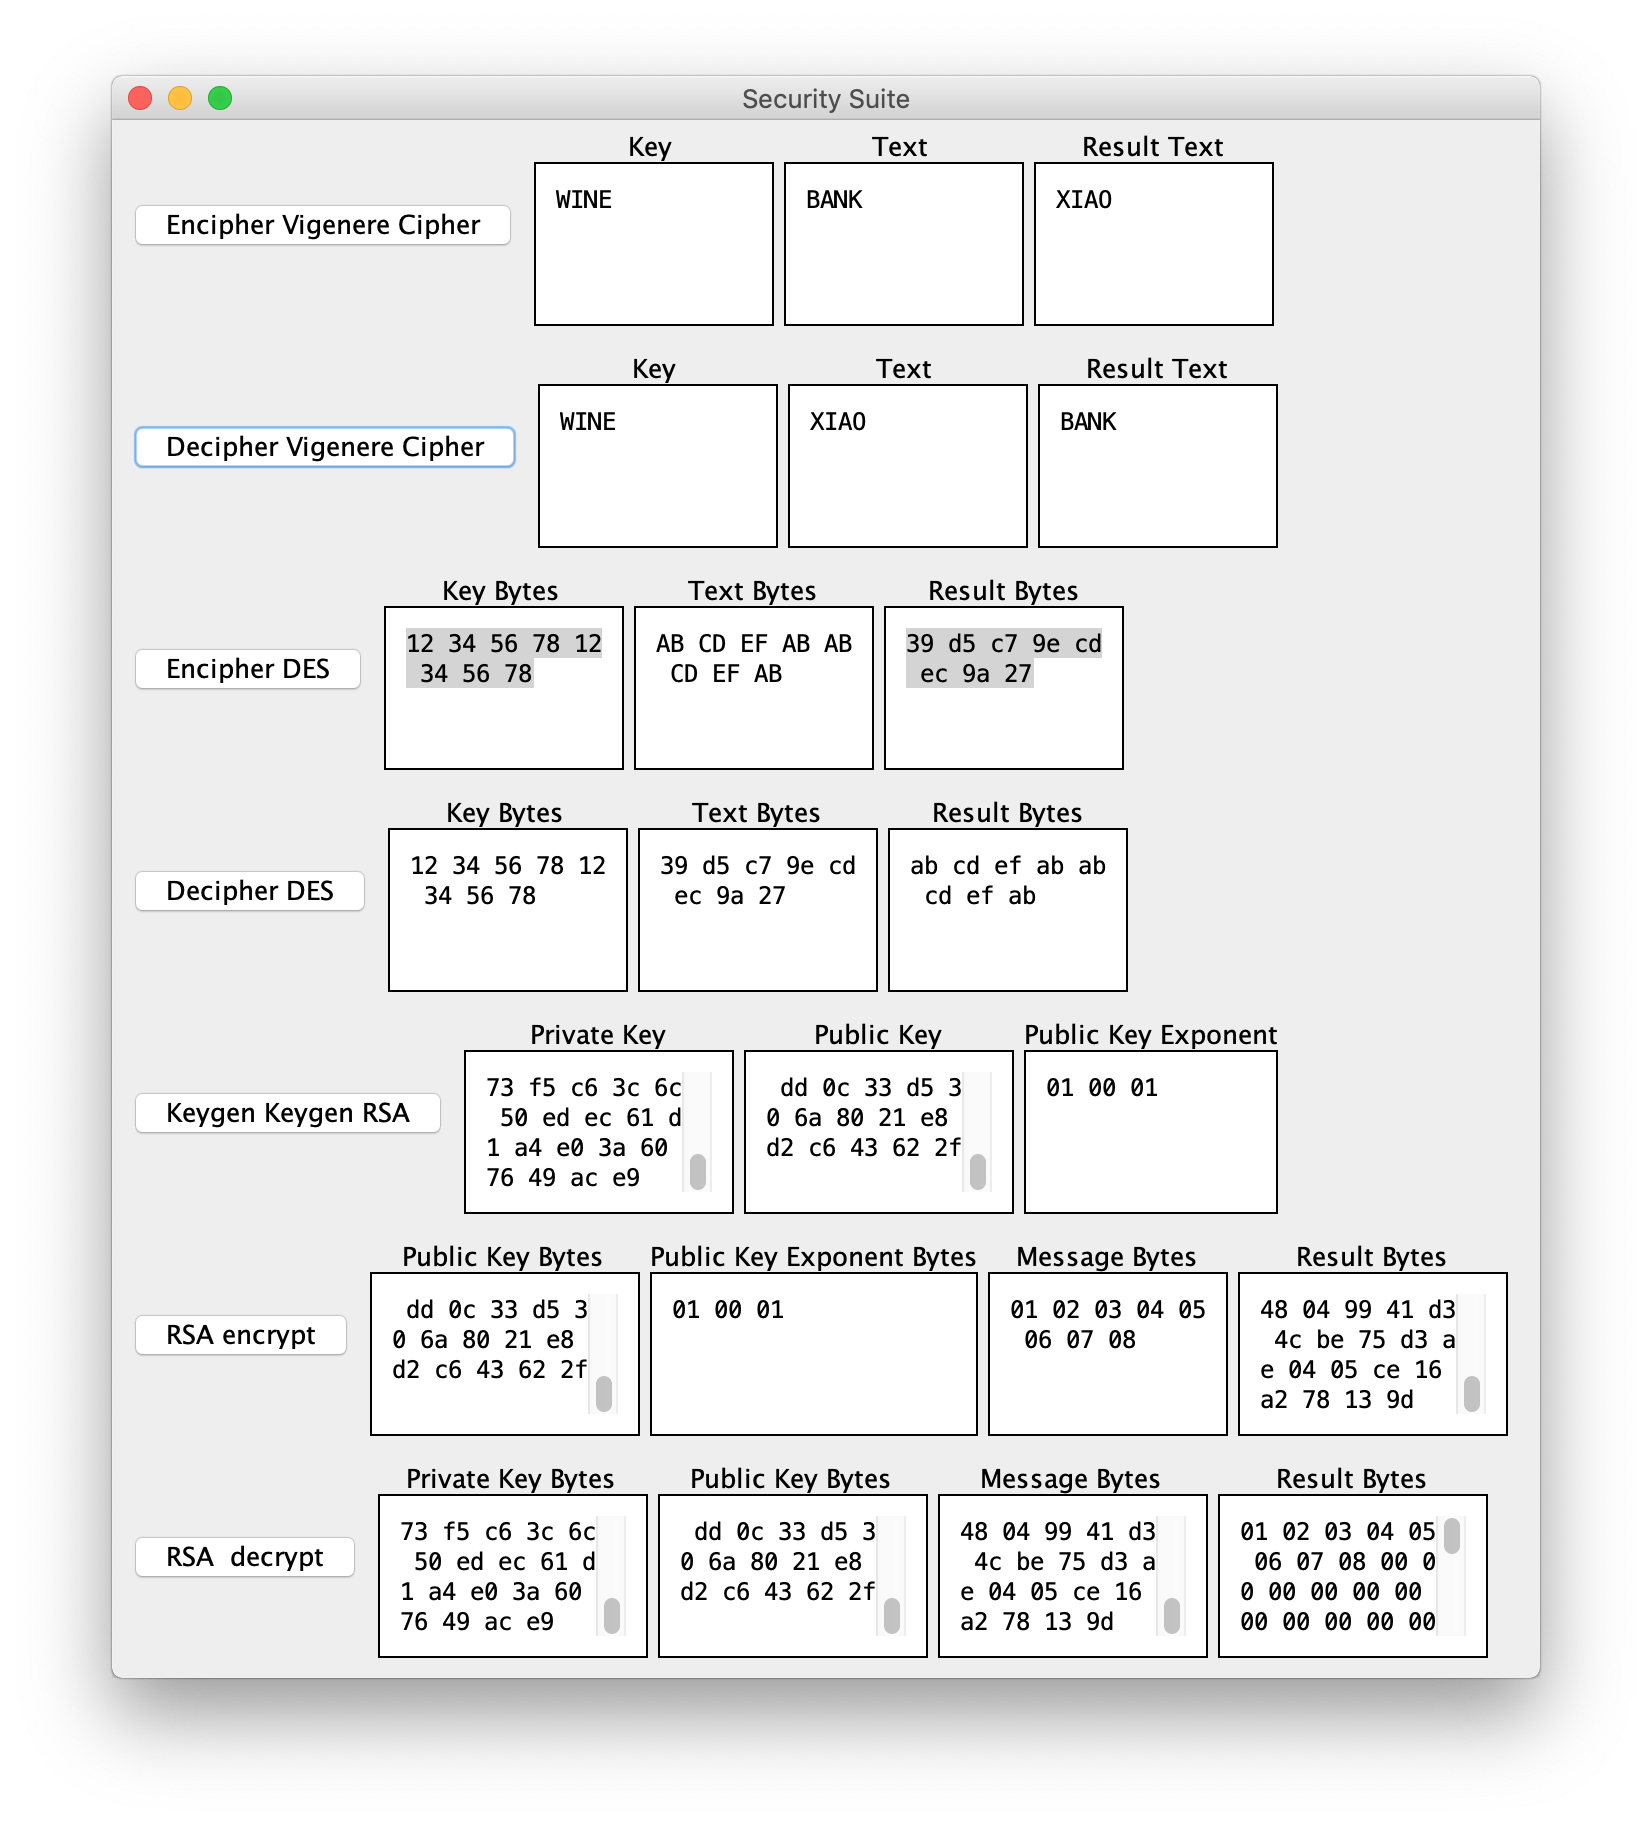
\includegraphics[scale=0.50]{demo}
  \Description{Image of our demo tool}
  \caption{Image of the security suite demo tool.}
  \label{fig:one}
\end{figure}

\subsection{Hashcat Demo}\label{sec:hashcat}

\textsc{Hashcat} is a software tool used to crack passwords, and can be used to leverage an available GPU for highly-parallelized general purpose computation. 

\section{Vigenère Cipher Cracker}\label{sec:vinegar}

Words go here too!

\section{Results}\label{sec:results}

Evaluation, efficiency? Challenges?

\section{Related Work}\label{sec:relatedwork}

Related work. Examples of citations with DOIs: \cite{2004:ITE:1009386.1010128, Kirschmer:2010:AEI:1958016.1958018}. Online citations: \cite{TUGInstmem, Thornburg01, CTANacmart}.

\section{Discussion}\label{sec:discussion}

What didn't we cover? :O

% Appendix
\appendix
\section{Elaboration on the ABCD algorithm}

This is an appendix, maybe about some equation
\begin{displaymath}
P=NP
\end{displaymath}

\section{Supplementary Materials}

\subsection{Hashcat materials}

Materials?

\subsection{Tool: Symmetric Ciphers Online }

\href{http://symmetric-ciphers.online-domain-tools.com/}{Link}

\begin{acks}

The authors would like to thank the mitochondria for being the powerhouse of the cell.

\end{acks}

% Bibliography
\bibliographystyle{ACM-Reference-Format}
\bibliography{sample-bibliography}

\end{document}
